%\documentclass{jsarticle}

%\usepackage{amsmath, amssymb}%数式
%\usepackage{array, booktabs}%表成型
%\usepackage[dvipdfmx]{graphicx}%画像

%\begin{document}

\subsection{プラスチックシンチレータのデータ解析}
\label{subsec:PSAnalyses}

\subsubsection{使用データ}
\label{subsubsec:PSData}
実験で得られたデータのうち,解析に用いたのは3 日目に磁場標的を用いたランと4 日目に銅板標的を用いたランとの2 つであり,それぞれ表\ref{tab:PSdata} のようなデータであった.
\begin{table}[h]
	\centering
	\caption{PS の解析に用いたデータ}
	\begin{tabular}{ccc} \toprule
	標的の種類 & 磁場$B~[\mathrm{Gauss}]$ & Event 数 \\ \midrule
	銅板標的 & --- & 43502 \\
	磁場標的 & 53.97 & 448073 \\ \bottomrule
	\end{tabular}\label{tab:PSdata}
\end{table}%

なお,磁場標的を用いたデータについては先に述べたように磁場がランの途中で変化していたので,解析には変化後のデータとして,最初の30000 Event を除いたデータのみを用いた.

\subsubsection{FADC 波形の解析}
\label{subsubsec:PSEventDisplay}
FADC (WaveDigitizer V1721) で得られたデータをプロットすると図\ref{fig:PSEventDisplayAll} のようになった.図\ref{fig:PSEventDisplayAll} は磁場標的を用いたランの1000 Event 目の波形であり,丸印はそれぞれの信号についてその点をピークとみなしたことを表す.ここでグラフの色はプラスチックシンチレータの各層に対応している(ただし3 層目にあたるch 4 はFinger Counter である).

\begin{figure}[h]
	\centering
	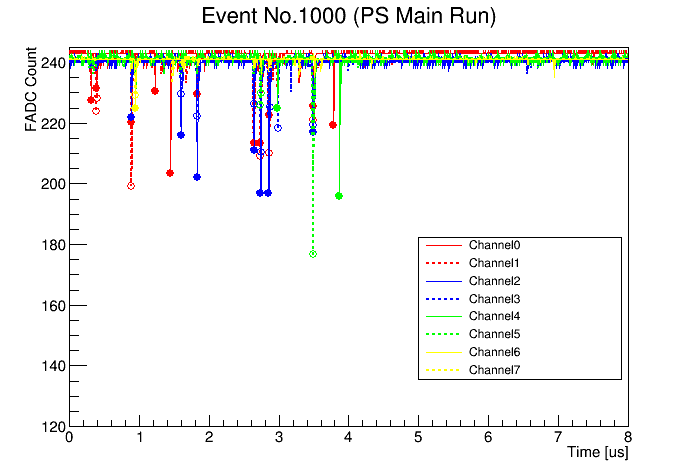
\includegraphics[width = 0.9\textwidth]{figure/odagawa/PSEventDisplayAll.png}
	\caption{プラスチックシンチレータで得られた波形($8~\mu\mathrm{s}$ 全体)}
	\label{fig:PSEventDisplayAll}
\end{figure}%

図\ref{fig:PSEventDisplayAll} の$2.6~\mu\mathrm{s}$ から$3.1~\mu\mathrm{s}$ までを拡大したものが図\ref{fig:PSEventDisplayZoom} である.

\begin{figure}[h]
	\centering
	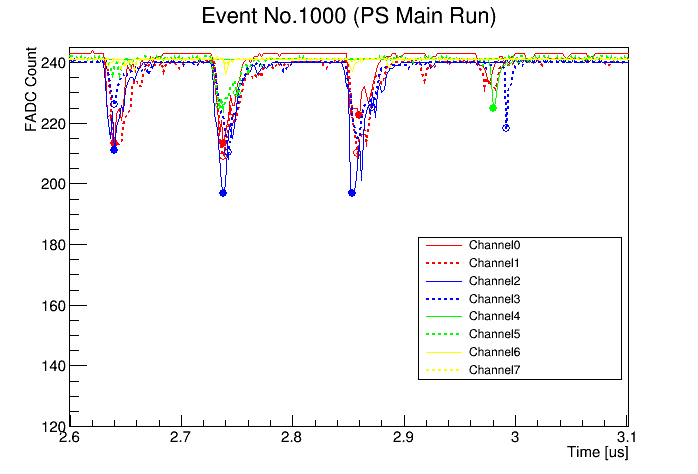
\includegraphics[width = 0.9\textwidth]{figure/odagawa/PSEventDisplayZoom.png}
	\caption{プラスチックシンチレータで得られた波形(一部拡大)}
	\label{fig:PSEventDisplayZoom}
\end{figure}%

図\ref{fig:PSEventDisplayZoom} からもわかる通り,プラスチックシンチレータの解析データについてはパイルアップの影響はほとんどないものと考えられる.また,信号の立ち下がりは十分早く,固定threshold 解析においてもTQ 補正などは必要ないと判断した.以降ではこれらを考慮したうえで,固定threshold を,プラスチックシンチレータのアフターパルスやベースラインの揺らぎを無視できる大きさ(8~FADC Count) に設定して解析を行った.

\subsubsection{ミュオン寿命解析}
\label{subsubsec:PSLife}
銅板標的を用いたランのデータの解析から,まずはミュオンの寿命を求めた.\ref{subsubsec:PSEventDisplay} で述べたようにthreshold を設定し,固定threshold を越えたところから初めて上回るところまでを一つの崩壊$e^{+}$ による信号として,threshold を超えた瞬間をその信号が持つ時間情報とした.その後,3 層目を除く各層については以下の方法でコインシデンスをとった.

各層について,時間情報が$10~\mathrm{ns}$ 以内にあれば同じ崩壊$e^{+}$ 由来の信号として,二つの平均時間を各層の時間情報とした.ここで$10~\mathrm{ns}$ という値は図\ref{fig:PSEventDisplayZoom} などからプラスチックシンチレータの立ち下がり時間程度になるように選んだ.

以上の時間情報を用いて実際に得られた3 層目を除く各層の時間情報ヒストグラムが図\ref{fig:PSLifeDist_Layer0} - \ref{fig:PSLifeDist_Layer3} である.ただし2, 4 層目は1 層目とのコインシデンスをとった.ここで3 層目を除いたのはチャンネル数の都合上,3 層目では層内でのコインシデンスをとることができなかったからである.また,コインシデンスをとった方法は各層での方法と同じであるが,時間情報としては1 層目と各層との平均を用いるのではなく,コインシデンスが取れたものを各層についてそのまま使用した.

\begin{figure}[h]
	\centering
	\begin{minipage}{0.45\textwidth}
	\centering
	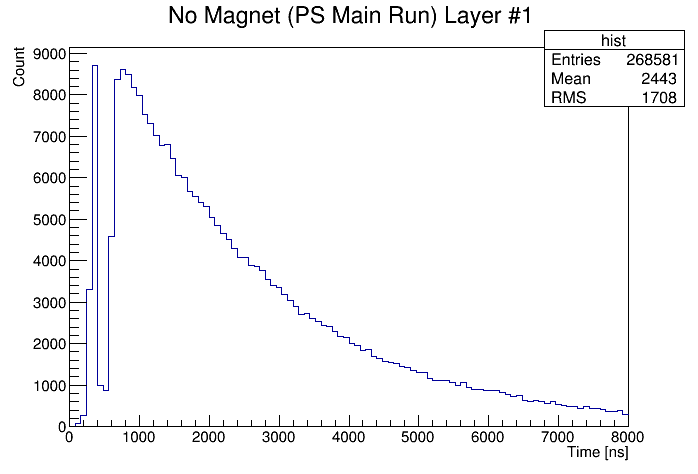
\includegraphics[width = \textwidth]{figure/odagawa/PSLifetimeDist_Layer0.png}
	\caption{磁場がないときの時間分布(1 層目)}
	\label{fig:PSLifeDist_Layer0}
	\end{minipage}
	\begin{minipage}{0.45\textwidth}
	\centering
	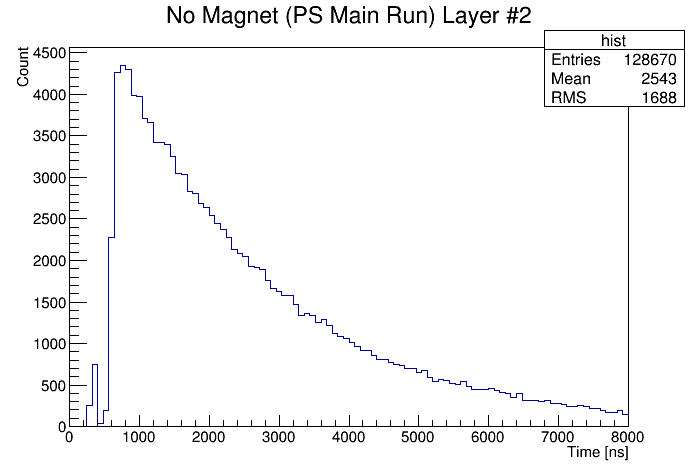
\includegraphics[width = \textwidth]{figure/odagawa/PSLifetimeDist_Layer1.png}
	\caption{磁場がないときの時間分布(2 層目)}
	\label{fig:PSLifeDist_Layer1}
	\end{minipage}
	\begin{minipage}{0.45\textwidth}
	\centering
	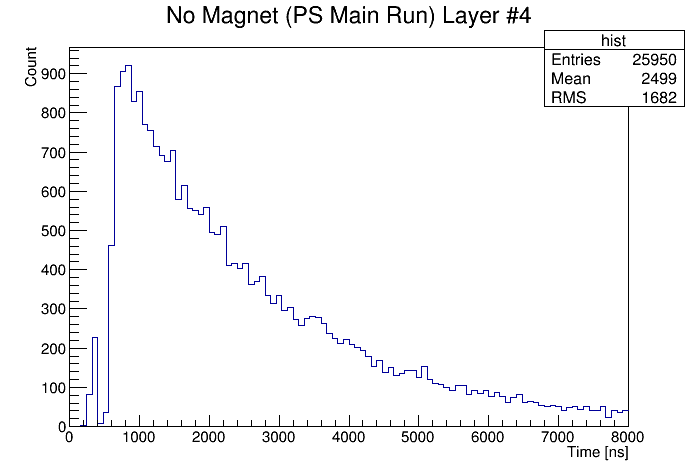
\includegraphics[width = \textwidth]{figure/odagawa/PSLifetimeDist_Layer3.png}
	\caption{磁場がないときの時間分布(4 層目)}
	\label{fig:PSLifeDist_Layer3}
	\end{minipage}
	\begin{minipage}{0.45\textwidth}
	\centering
	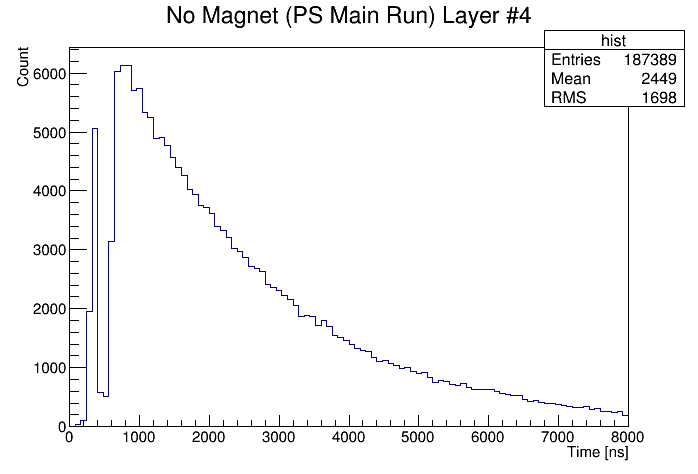
\includegraphics[width = \textwidth]{figure/odagawa/PSLifetimeDistNoCoin_Layer3.png}
	\caption{磁場がないときの時間分布(4 層目,コインシデンスなし)}
	\label{fig:PSLifeDistNoCoin_Layer3}
	\end{minipage}
\end{figure}%

得られた時間分布について,まず早いところにピークが立っている.このピークは図\ref{fig:PSLifeDist_Layer3}, \ref{fig:PSLifeDistNoCoin_Layer3} を比較すると分かるように,コインシデンスをとることによって小さくなる.このピークは$\pi$ の崩壊によってできた表面ミュオンがすぐに崩壊し,生成した$e^{+}$ が,ビームラインを通り抜けて直接検出器に当たったときの信号によるものと考えられる.ビームラインにおいては運動量で粒子を選択しており(今回は$4.1~\mathrm{MeV}$ の粒子を選択している),このようにしてできた$e^{+}$は同じ運動量の$\mu^{+}$ よりも高速で検出器に到達する.1 層目とのコインシデンスをとることでこのピークが低くなるのは,このコインシデンスにより粒子の飛来した方向を制限でき,銅板標的由来の信号の割合が多くなるためと考えられる.

図\ref{fig:PSLifeDist_Layer0} - \ref{fig:PSLifeDist_Layer3} のヒストグラムに式\eqref{eq:PSLifeFitFunc} で表される関数$f(t)$を用いてフィッティングを行った.ここでバックグラウンドの影響を加味して定数項を加え,フィッテイング範囲は1000~ns から8000~ns とした.フィッティング結果が図\ref{fig:PSLifeFit_Layer0} - \ref{fig:PSLifeFit_Layer3} ,および表\ref{tab:PSLifetime} である.統計誤差はROOT のフィッティングによるものである.

\begin{equation}
f(t) = A \exp(-t / \tau) + \mathrm{const.}
\label{eq:PSLifeFitFunc}
\end{equation}

\begin{figure}[h]
	\centering
	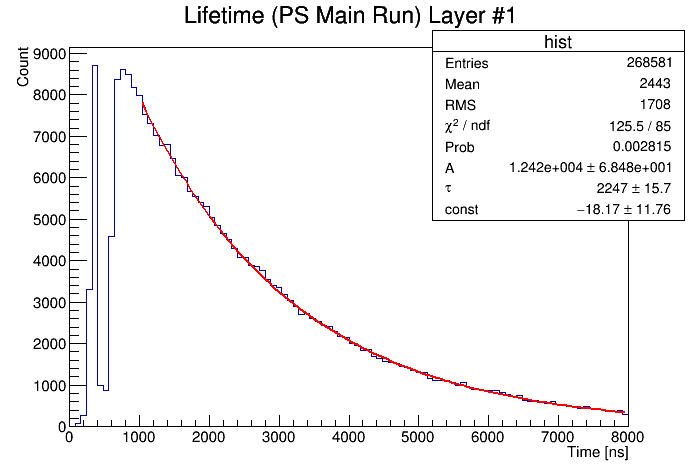
\includegraphics[width = 0.45\textwidth]{figure/odagawa/PSLifetimeFit_Layer0.png}
	\caption{ミュオン崩壊寿命フィッティング結果(1 層目)}
	\label{fig:PSLifeFit_Layer0}
	\begin{minipage}{0.45\textwidth}
	\centering
	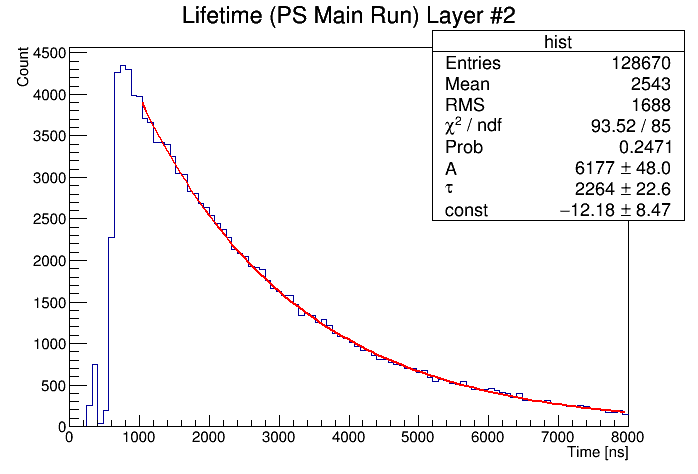
\includegraphics[width = \textwidth]{figure/odagawa/PSLifetimeFit_Layer1.png}
	\caption{ミュオン崩壊寿命フィッティング結果(2 層目)}
	\label{fig:PSLifeFit_Layer1}
	\end{minipage}
	\begin{minipage}{0.45\textwidth}
	\centering
	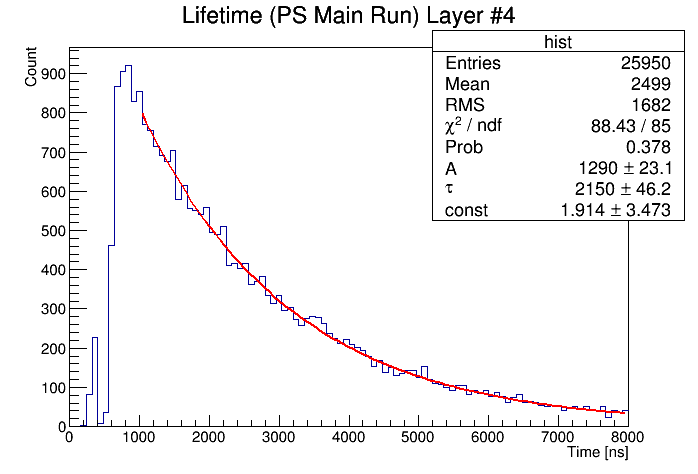
\includegraphics[width = \textwidth]{figure/odagawa/PSLifetimeFit_Layer3.png}
	\caption{ミュオン崩壊寿命フィッティング結果(4 層目)}
	\label{fig:PSLifeFit_Layer3}
	\end{minipage}
\end{figure}%

\begin{table}[h]
	\centering
	\caption{フィッティングによって得られた$\tau$ の値}
	\begin{tabular}{cc}\toprule
	層番号 & $\tau~[\mathrm{ns}]$ \\ \midrule
	1 & $2247 \pm 16$ \\
	2 & $2264 \pm 23$ \\
	4 & $2150 \pm 46$ \\ \bottomrule
	\end{tabular}\label{tab:PSLifetime}
\end{table}%

\newpage

\subsubsection{ミュオン$g$ 因子解析}
\label{subsubsec:PSgFactor}
次に磁場標的を用いたランの解析から,ミュオンの$g$ 因子を求めた.ここで先述の通り,磁場の変化を確認した結果から,最初の30000~Events を除いたデータを用いた.\ref{subsubsec:PSLife} と同様に時間情報を求めて図\ref{fig:PSgFactorDist_Layer0} - \ref{fig:PSgFactorDist_Layer3} のようなヒストグラムを得た.

\begin{figure}[h]
	\centering
	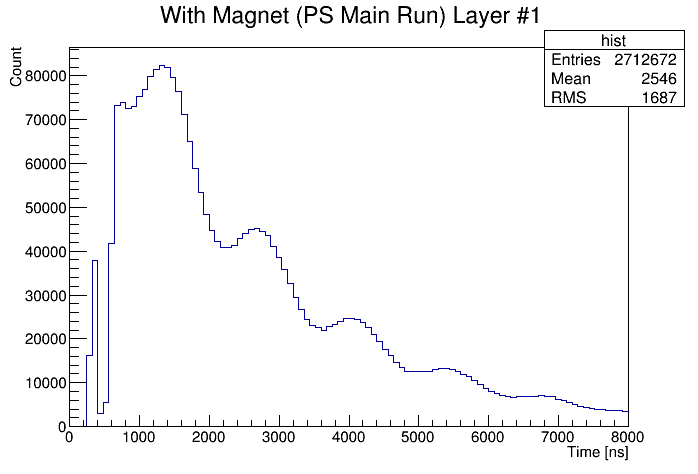
\includegraphics[width = 0.45\textwidth]{figure/odagawa/PSgFactorDist_Layer0.png}
	\caption{磁場があるときの時間分布(1 層目)}
	\label{fig:PSgFactorDist_Layer0}
	\begin{minipage}{0.45\textwidth}
	\centering
	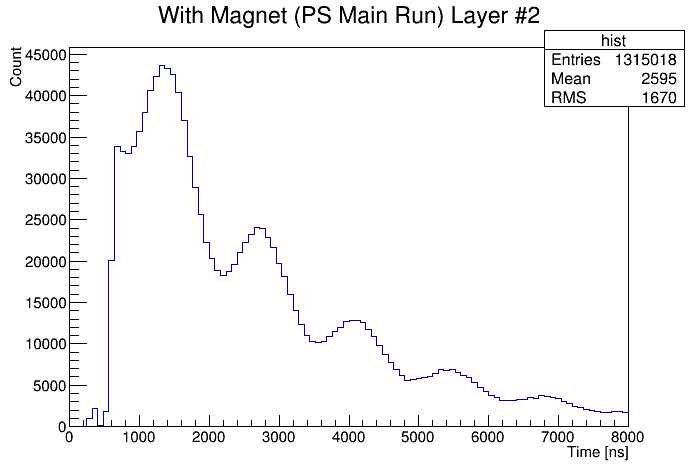
\includegraphics[width = \textwidth]{figure/odagawa/PSgFactorDist_Layer1.png}
	\caption{磁場があるときの時間分布(2 層目)}
	\label{fig:PSgFactorDist_Layer1}
	\end{minipage}
	\begin{minipage}{0.45\textwidth}
	\centering
	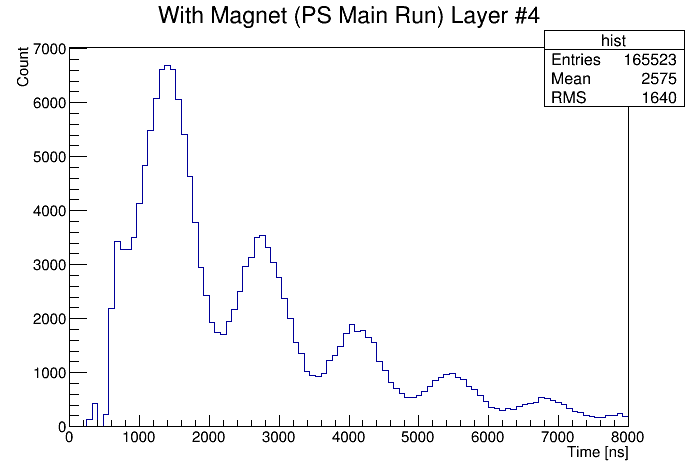
\includegraphics[width = \textwidth]{figure/odagawa/PSgFactorDist_Layer3.png}
	\caption{磁場がないときの時間分布(4 層目)}
	\label{fig:PSgFactorDist_Layer3}
	\end{minipage}
\end{figure}%

図\ref{fig:PSgFactorDist_Layer0} - \ref{fig:PSgFactorDist_Layer3} のヒストグラムに式\eqref{eq:PSgFactorFitFunc} で表される関数$g(t)$ を用いてフィッティングを行った.ここで\ref{subsubsec:PSLife} のときと同様に定数項を加え,フィッティング範囲も振動がきちんと見えている1000~ns から8000~ns までとした.フィッティング結果は図\ref{fig:PSgFactorFit_Layer0} - \ref{fig:PSgFactorFit_Layer3},および表\ref{tab:PSgFactor} となった.ただし表\ref{tab:PSgFactor} において$g$ 因子の計算には各点の磁場をビームプロファイルのガウシアンで加重平均した値,$B = 53.97~[\mathrm{Gauss}]$ という値を用いた.また,統計誤差としては\ref{subsubsec:PSLife} と同様にROOT のフィッティングによって得られたものを載せており,磁場の影響を含めたものについては後述する.

\begin{equation}
g(t) = A \exp(-t / \tau) [1 + B \cos(\delta + \omega t)] + \mathrm{const.}
\label{eq:PSgFactorFitFunc}
\end{equation}

\begin{figure}[h]
	\centering
	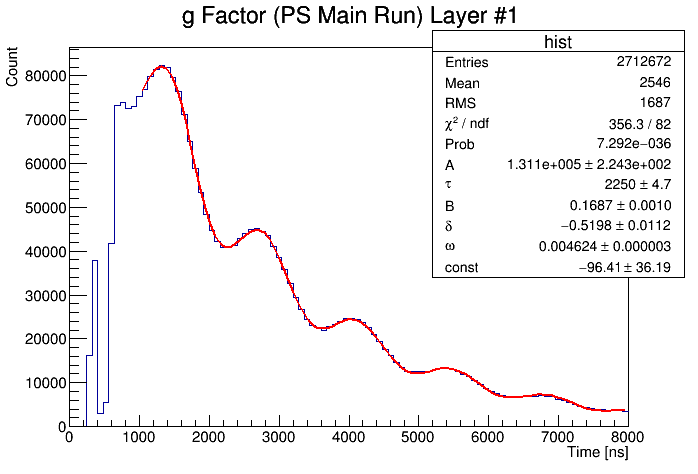
\includegraphics[width = 0.45\textwidth]{figure/odagawa/PSgFactorFit_Layer0.png}
	\caption{ミュオン$g$ 因子フィッティング結果(1 層目)}
	\label{fig:PSgFactorFit_Layer0}
	\begin{minipage}{0.45\textwidth}
	\centering
	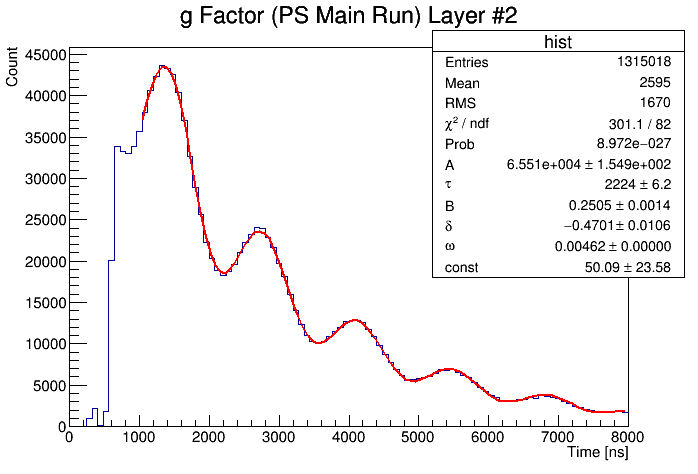
\includegraphics[width = \textwidth]{figure/odagawa/PSgFactorFit_Layer1.png}
	\caption{ミュオン$g$ 因子フィッティング結果(2 層目)}
	\label{fig:PSgFactorFit_Layer1}
	\end{minipage}
	\begin{minipage}{0.45\textwidth}
	\centering
	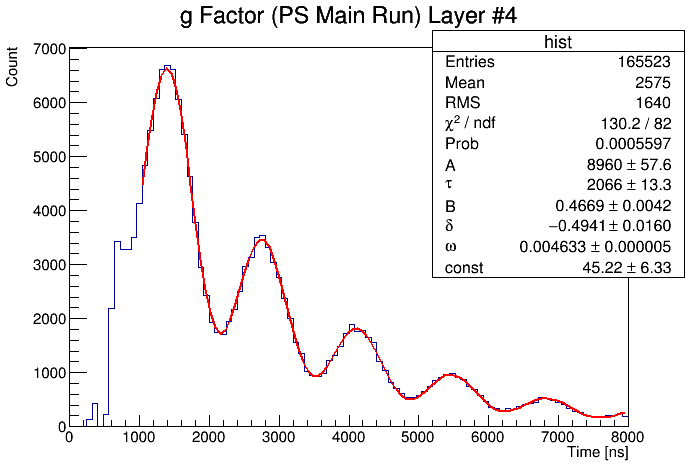
\includegraphics[width = \textwidth]{figure/odagawa/PSgFactorFit_Layer3.png}
	\caption{ミュオン$g$ 因子フィッティング結果(4 層目)}
	\label{fig:PSgFactorFit_Layer3}
	\end{minipage}
\end{figure}%

\begin{table}[h]
	\centering
	\caption{$g$ 因子フィッティング結果}
	\begin{tabular}{cccc} \toprule
	層番号 & $\tau~[\mathrm{ns}]$ & $\omega~[/ \mu\mathrm{s}]$ & $g$ \\ \midrule
	1 & $2249 \pm \phantom{0}4$ & $4.624 \pm 0.004$ & $2.013 \pm 0.0015$ \\  
	2 & $2224 \pm \phantom{0}6$ & $4.620 \pm 0.003$ & $2.012 \pm 0.0015$ \\  
	4 & $2066 \pm 13$ & $4.633 \pm 0.005$ & $2.017 \pm 0.0023$ \\  \bottomrule
	\end{tabular}\label{tab:PSgFactor}
\end{table}%

\newpage

\subsubsection{磁場の系統誤差について}
\label{subsubsec:MagSysErr}
\ref{subsubsec:PSgFactor} において$g$ 因子解析に用いた磁場の値$B = 53.97~[\mathrm{Gauss}]$ は事前にMLF の三宅さんから頂いたビームプロファイルをもとに加重平均をとった値であるが,このビームプロファイルの不定性により加重平均の値は変化する.今回はビームの広がりはガウシアンに乗ると仮定したうえでガウシアンの広がりを変化させ,それによって現れる磁場,および$g$ 因子の系統誤差をみた.

ガウシアンの$x$ 方向の広がりを$\sigma_{x}$,$y$ 方向の広がりを$\sigma_{y}$ とし,$\sigma_{x}$ を2.0~cm から3.9 ~cm まで,$\sigma_{y}$ を1.0~cm から2.9~cm まで0.1~cm 刻みで変化させて加重平均磁場の値を求めたところ磁場の最大値・最小値は表\ref{tab:MagSysErr} のようになった.ここで$\sigma_{x}, \sigma_{y}$ を動かす範囲は磁場標的の大きさが標準偏差$1\sigma$ に入る点を上限として十分な広さをとった.

\begin{table}[h]
	\centering
	\caption{$\sigma_{x}$,$\sigma_{y}$を動かしたときの磁場$B$ の最大値と最小値~[Gauss]}
	\begin{tabular}{cc}\toprule
	$B_{\mathrm{max}}$ & $B_{\mathrm{min}}$ \\ \midrule
	$54.44 (\sigma_{x} = 3.9, \;\sigma_{y} = 1.0)$ & $53.76 (\sigma_{x} = 3.9,\;\sigma_{y} = 2.9)$ \\ \bottomrule 	
	\end{tabular}\label{tab:MagSysErr}
\end{table}%

得られた磁場の最大値,および最小値を用いて$g$ 因子を計算すると表\ref{tab:PSgSysErr} のような値がそれぞれ得られた.

\begin{table}[h]
	\centering
	\caption{磁場$B$ の値とそれらに対応する$g$ 因子の値}
	\begin{tabular}{cccc}\toprule
	層番号 & $B_{\mathrm{max}} = 54.44$ & $B_{0} = 53.97$ & $B_{\mathrm{min}} = 53.76$ \\ \midrule
	1 & 2.000 & 2.013 & 2.021 \\
	2 & 1.995 & 2.012 & 2.020 \\
	4 & 2.000 & 2.017 & 2.025 \\ \bottomrule 
	\end{tabular}\label{tab:PSgSysErr}
\end{table}%

また,磁場の測定誤差を含んだ$g$ 因子の統計誤差については,誤差伝播の式,式\eqref{eq:PSgosa} を用いて計算した.$\delta B = 0.008~\mathrm{Gauss}$となったので,$\delta g$ は表\ref{tab:PSgStatErr} のようになった.

\begin{equation}
\delta g = \sqrt{\left(\delta\omega\right)^{2}\left(\frac{\partial g}{\partial\omega}\right)^{2} + \left(\delta B\right)^{2}\left(\frac{\partial g}{\partial B}\right)^{2}}
\label{eq:PSgosa}
\end{equation}%

\begin{table}
	\centering
	\caption{磁場の測定誤差を含んだ$g$ 因子の統計誤差}
	\begin{tabular}{cc}\toprule
	層番号 & $g$ 因子の統計誤差\\ \midrule
	1 & 0.0016 \\ 
	2 & 0.0015 \\
	4 & 0.0023 \\ \bottomrule
	\end{tabular}\label{tab:PSgStatErr}
\end{table}%

実際,$g$ 因子の値を考えるときは1 層目と4 層目とのコインシデンスをとったものが貫通イベントをとれている可能性が高く妥当であると考えると,得られた$g$ 因子の値は
\[g = 2.017 \pm 0.0023 ^{+0.008}_{-0.017}\]
となった.ここで誤差の第一項は磁場の影響を含めた統計誤差であり,第二項はビームプロフィルの不定性による系統誤差である.

%以下二つはAppendix にまわす?
%%%%%%%%%%%%%%%
\subsubsection{磁場の変化の確認}
\label{subsubsec:PSMagChangeCheck}
$g$ 因子測定のための磁場標的を置いたランの途中において,磁石配置が崩れ磁場の値などが変わっていたことは本文中でも述べたが解析においてそのことを確認した.

\ref{subsubsec:PSgFactor} のようなフィッティングをする際に,用いるイベントを9000~Events (6~min) ごとに区切ってフィッティングを行い,それぞれ$\omega$ を求めると図\ref{fig:PSOmegaCheck} のようになった.また図\ref{fig:PSCycleCheck} はそれぞれを振動周期に直したものである.赤線は最初の8~分間のデータのみがたまたまあったのでそこから得られた値を表しており,また青線は磁場変化発覚後に改めて確認用にとったランから得られた値を表している.図\ref{fig:PSOmegaCheck}, \ref{fig:PSCycleCheck} を見ると分かるように,ランの最初の20~分程度で磁場の値が変化していることが分かる.よって今回の解析には同じ値の磁場とみなせるという条件の下で,より統計量の多いランの20~分以降のデータを用いることにした.なお,変化前後の加重平均をとった磁場の値はそれぞれ56.06~Gauss と53.97 Gauss であった.

\begin{figure}[h]
	\centering
	\begin{minipage}{0.45\textwidth}
	\centering
	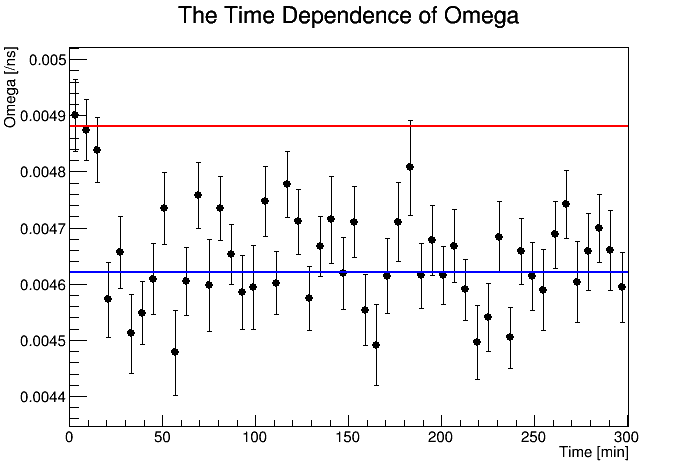
\includegraphics[width = \textwidth]{figure/odagawa/PSOmegaCheck.png}
	\caption{ラン中における$\omega$ の時間変化}
	\label{fig:PSOmegaCheck}
	\end{minipage}
	\begin{minipage}{0.45\textwidth}
	\centering
	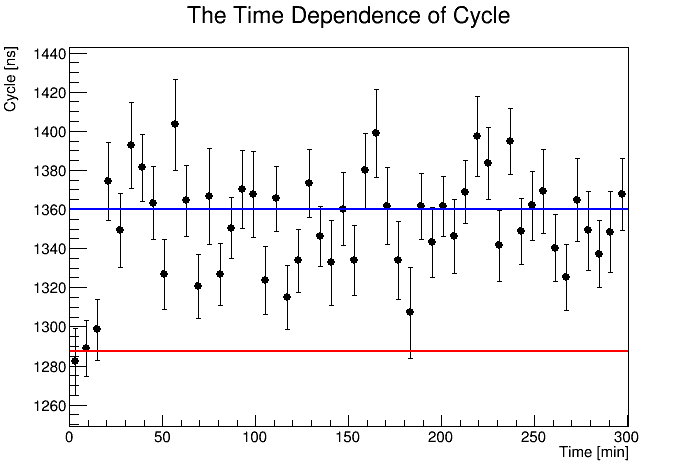
\includegraphics[width = \textwidth]{figure/odagawa/PSCycleCheck.png}
	\caption{ラン中における振動周期 の時間変化}
	\label{fig:PSCycleCheck}
	\end{minipage}
\end{figure}

\subsubsection{NaI シンチレータとの位相差の確認}
\label{subsubsec:PhaseCheck}
NaI シンチレータとプラスチックシンチレータの$g$ 因子の解析から$\cos$ 振動の初期位相$\delta$ に注目すると,これら二つの位相差は実験中の物理的セットアップに起因していると考えられる.実際,二つのシンチレータは標的に対しておよそ$87^{\circ}$ の角度をつけて配置していたため,それにともなって初期位相もおよそ$87^{\circ}$ 分の差をもっているはずである.

これらの事実を解析から確かめるために,まず二つの検出器から得られたデータの時間原点をそろえる必要がある.これら二つの検出器では検出器の性能差もあるが,そもそも用いたケーブルの長さが違うために時間原点がそろっていない.今回は時間原点をそろえるために\ref{subsubsec:PSLife} でものべた高速$e^{+}$ 粒子による小さなピークをそろえることを考えた.ビームライン奥からミュオンに比べて高速で飛んでくる$e^{+}$ は,今回のセットアップにおいては二つの検出器にほぼ同様の時間かけて飛んでくるはずなので,このピークをそろえることで時間原点とすることができる.図\ref{fig:NaITimeOrigin}がNaI シンチレータの$e^{+}$ ピーク探索とそれを用いた原点調整後のヒストグラム,図\ref{fig:PSTimeOrigin} はプラスチックシンチレータで同様のことを行ったものである.

\begin{figure}[h]
	\centering
	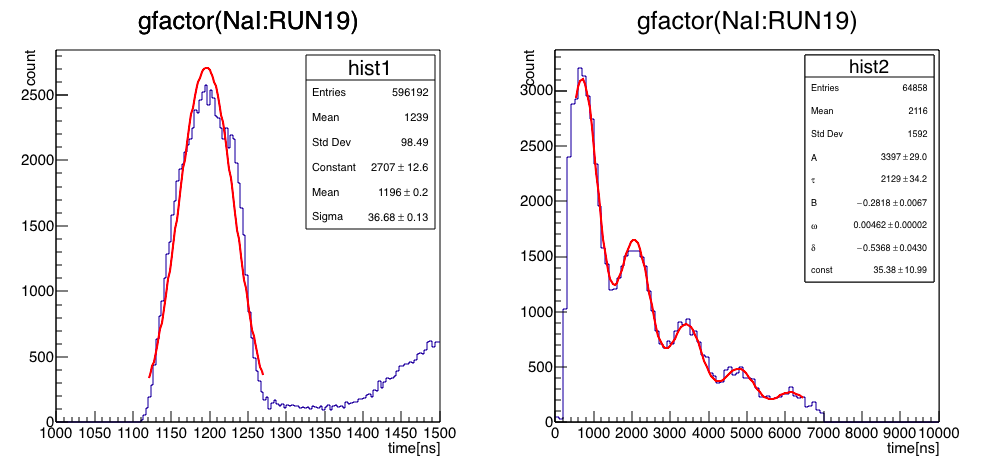
\includegraphics[width = 0.9\textwidth]{figure/odagawa/NaITimeOrigin.png}
	\caption{NaI シンチレータにおける時間原点探索と原点調節後のヒストグラム}
	\label{fig:NaITimeOrigin}
	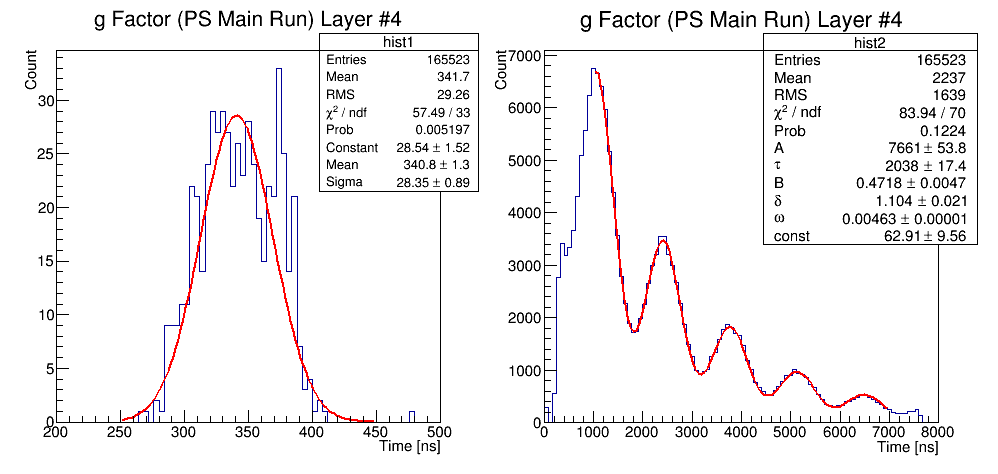
\includegraphics[width = 0.9\textwidth]{figure/odagawa/PSTimeOrigin.png}
	\caption{プラスチックシンチレータにおける時間原点探索と原点調節後のヒストグラム}
	\label{fig:PSTimeOrigin}
\end{figure}

それぞれのフィッティングから得られた初期位相$\delta$ は表\ref{tab:InitPhases} のようになった.

\begin{table}[h]
	\centering
	\caption{各検出器の初期位相}
	\begin{tabular}{cc}\toprule
	検出器 & $\delta$ \\ \midrule
	NaI シンチレータ & $-0.54 \pm 0.04$ \\
	プラスチックシンチレータ & $\phantom{-}1.10 \pm 0.02$ \\ \bottomrule
	\end{tabular}\label{tab:InitPhases}
\end{table}%
したがって,表\ref{tab:InitPhases} からもわかるとおり位相差は$1.64 \pm 0.06 \sim \pi / 2$ となりセットアップの角度と整合していることが確認できた.
%%%%%%%%%%%%%%%
%\end{document}
